\section{Plots}

In this section, we want to focus on different examples of plots.  We restrict
our presentation to \toolname{pgfplots} because it is the tool we use most;
every example can be done with the other tools, respectively.  The raw data that
is used in the examples can be found in the supplementary GitHub
repository\footnoteref{footnote-github} and on the supplementary web
page\footnoteref{footnote-webpage}.

A good idea before starting with the plot generation is to think about the type
of plot that should be used and the colors in it.  Together with the
\toolname{pgfplots} package comes a library called \emph{colorbrewer}; this
library bundles several color schemes for an easy use.  Before choosing one,
one should think about where the plot will be used—printing often requires
different colors than presentation slides.  Nonetheless, in both cases all plots
should be made of the same color scheme.  Information about the available
schemes can be found in the \toolname{pgfplots}
manual~\cite[Sect.~5.2]{Feuersaenger2016}.

\subsection{Bar Plots}

We start with a first plot by creating a simple bar plot.  In our example we
have a number of values that should be printed and put these numbers directly
into the code that creates the plot instead of loading them from, for example, a
CSV file.  The code that is necessary to create such a simple plot can be seen
in Listing~\ref{lst:barplot}; the output can be seen in
Figure~\ref{fig:barplot}.

When looking at the code, one will notice the settings in lines 8 to 15.  Most
of them are not necessary to create the plot; they are only used to make the
output look more beautiful.  We refer the reader to the documentation of
\toolname{pgfplots}~\cite{Feuersaenger2016} for further information and more
options that can be used for improving the style of the plot.

The bar plot is a very simple and effective way to present a small amount of
data.  One can imagine that for a large number of values, the bar plot will get
confusing.  Especially labels of the bars will be difficult to read when printed
in a very small font.

\begin{listing}[H]
  \inputminted{latex}{../examples/barplot.tex}
  \caption{Code example to create the bar plot in Fig.~\ref{fig:barplot}}
  \label{lst:barplot}
\end{listing}
\begin{figure}[!t]
  \centering
  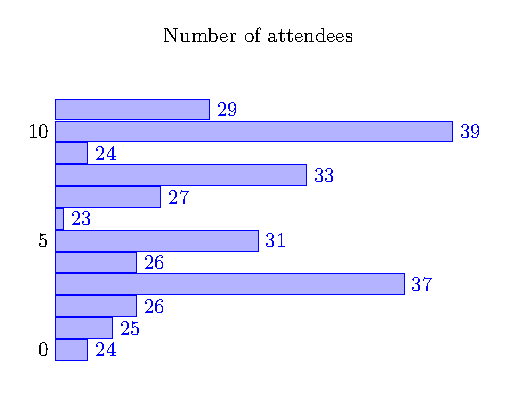
\includegraphics{barplot}
  \caption{Bar plot created from the code in Lst.~\ref{lst:barplot}}
  \label{fig:barplot}
\end{figure}

\subsection{Scatter Plots}

A scatter plot is a two dimensional (more are possible, however) plot using
cartesian coordinates to display values.  It can be used, for example, to show
the correlation between data.

Consider students that write an exam as an example.  During the lecture time,
the students had the possibility to work on tasks for homework and hand in their
solutions for correction.  For each of these homework tasks, a student can get
points.  These points are summed up for every student (and for simplicity saved
as the percentage of achieved points to total points).  The same is done for the
points a student achieved in the exam.  We now have two data values for each
student: points achieved in homework and points achieved in exam.  We can now
easily put a marker for each student in a two dimensional grid using points in
homework as one axis and point in exam as the other.

An example code that creates such a plot can be found in
Listing~\ref{lst:scatterplot}; the output can be seen in
Figure~\ref{fig:scatterplot}.

\begin{listing}[H]
  \inputminted{latex}{../examples/scatterplot.tex}
  \caption{Code example to create a scatter plot from a CSV}
  \label{lst:scatterplot}
\end{listing}

\begin{figure}[!t]
  \centering
  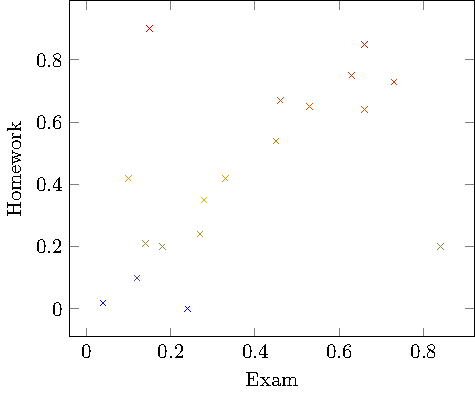
\includegraphics{scatterplot}
  \caption{Scatter plot created from the code in Lst.~\ref{lst:scatterplot}}
  \label{fig:scatterplot}
\end{figure}

\subsection{Quantile Plots}

\subsection{Automatic Generation with \hologo{LuaLaTeX}}

With the \TeX{} engine \hologo{LuaTeX}, which combines \hologo{pdfTeX} with
OpenType and Unicode support, \hologo{METAPOST}, and Lua, it is possible to
generate tables or plots from input data while using a simple scripting
language.  Although this is also possible with plain \TeX{}, it might be more
convenient to program in a scripting language rather than \TeX{}.  The example
in Table~\ref{tab:lualatex-autogenerated} is generated from a CSV file that was
exported by the unit test coverage report of IntelliJ IDEA.

\begin{luacode}
tex.print("\\begin{table}[!t]")
tex.print("\\centering")
tex.print("\\caption{Autogenerated table with \\hologo{LuaLaTeX}}")
tex.print("\\label{tab:lualatex-autogenerated}")
tex.print("\\begin{tabular}{@{}l"
  .. "S[table-format=2.2,round-mode=figures,round-precision=4]r"
  .. "r@{}}")
tex.print("\\textbf{Package} & \\textbf{Line} & \\textbf{\\#} & \\\\\\midrule")

local zeile, daten
for zeile in io.lines("../examples/coverage-unittests-model-line-coverage.csv") do
  daten = fromCSV(zeile)
  local linepercent, linebar, pkgname
  pkgname = daten[1]
  linepercent = string.format("%.2f", daten[6] / daten[7] * 100)
  linebar = tonumber(string.format("%.4f", daten[6] / daten[7]))

  tex.print("" .. pkgname .. "&"
    .. linepercent .. "\\,\\% & (" .. daten[6] .. "/" .. daten[7] .. ")&"
    .. "\\begin{tikzpicture}"
    .. "\\draw [black,thin] (0,0) rectangle (1.0,0.15);"
    .. "\\tikz \\fill [gruen] (0,0) rectangle (" .. linebar .. ",0.15);"
    .. "\\tikz \\fill [rot] (" .. linebar .. ",0) rectangle (1.0,0.15);"
    .. "\\end{tikzpicture}"
    .. "\\\\")
end

tex.print("\\end{tabular}")
tex.print("\\end{table}")
\end{luacode}

Obviously, this data can change during the development of an application; one
does not want to adjust the table by hand, every time the coverage data changes.
Therefore, we simply parse the CSV file and create the table using
\hologo{LuaTeX}.  An example code for doing this, can be found in
Listing~\ref{lst:lua-autofilled-table}.

\begin{listing}[H]
  \inputminted[firstline=22,lastline=54]{latex}{../examples/lua-autofilled-table.tex}
  \caption{Code snippet to automatically generate a table like
    Table~\ref{tab:lualatex-autogenerated} with \hologo{LuaLaTeX}}
  \label{lst:lua-autofilled-table}
\end{listing}
